\section{Methodology}\label{sec:methodology}
\subsection{Data gathering}
In order to analyse the salmon price, we first need to gather this data on the salmon price. The main data point is the price of salmon. There are several sources for this data, but we utilized the data from the NASDAQ salmon exchange. The reason for this being a combination of the accessibility of the data, and the fact that the NASDAQ salmon exchange (NQSALMON) uses a weighted average for the salmon price, gathered from a spectrum of salmon exporters and it is therefore the best source of meaningful data. Another reason for using the NASDAQ salmon exchange is that the data is updated weekly with no missing values for the entire time frame. We downloaded data from March 2013 through December 2022, for a total of 507 data points. This was our base for the independent factors. The next step was to gather data from the other relevant factors for our analysis.

\subsection{Descriptive analysis}
\subsubsection{Salmon Price}\label{Salmon Price}
By looking at some simple descriptive statistics we will be able to decern if there are any changes needed to be done in the pre-processing stage. We will also examine if there are any trends or correlations that we will have to capture in order to produce the models. Let us begin by looking at our main variable, the salmon price.

\begin{figure}[H]
    \centering
    \includegraphics[width=0.8\textwidth]{data/Figures/Descriptive/SalmonPricePlot.png}
    \caption[Evolution of the salmon price]{Salmon price evolution.}\label{fig: Salmon price evolution}
\end{figure}

Looking at the plot we can see that the price has been increasing over the years. The top price having tripled our starting price, the mean of the price seems to have risen as well. Another increase we notice is the increasing magnitude of the price fluctuation. This is not only causing out highest prices but also some of the lowest prices in recent year. The plot is also showing the seasonal pattern that we expected to find in the price data where it is higher in the winter and lower in the summer. This is a characteristic we want our models to capture in order to make more precise predictions. To understand the seasonality of the price better we plot the prices for each month of the year.

\begin{figure}[H]
    \centering
    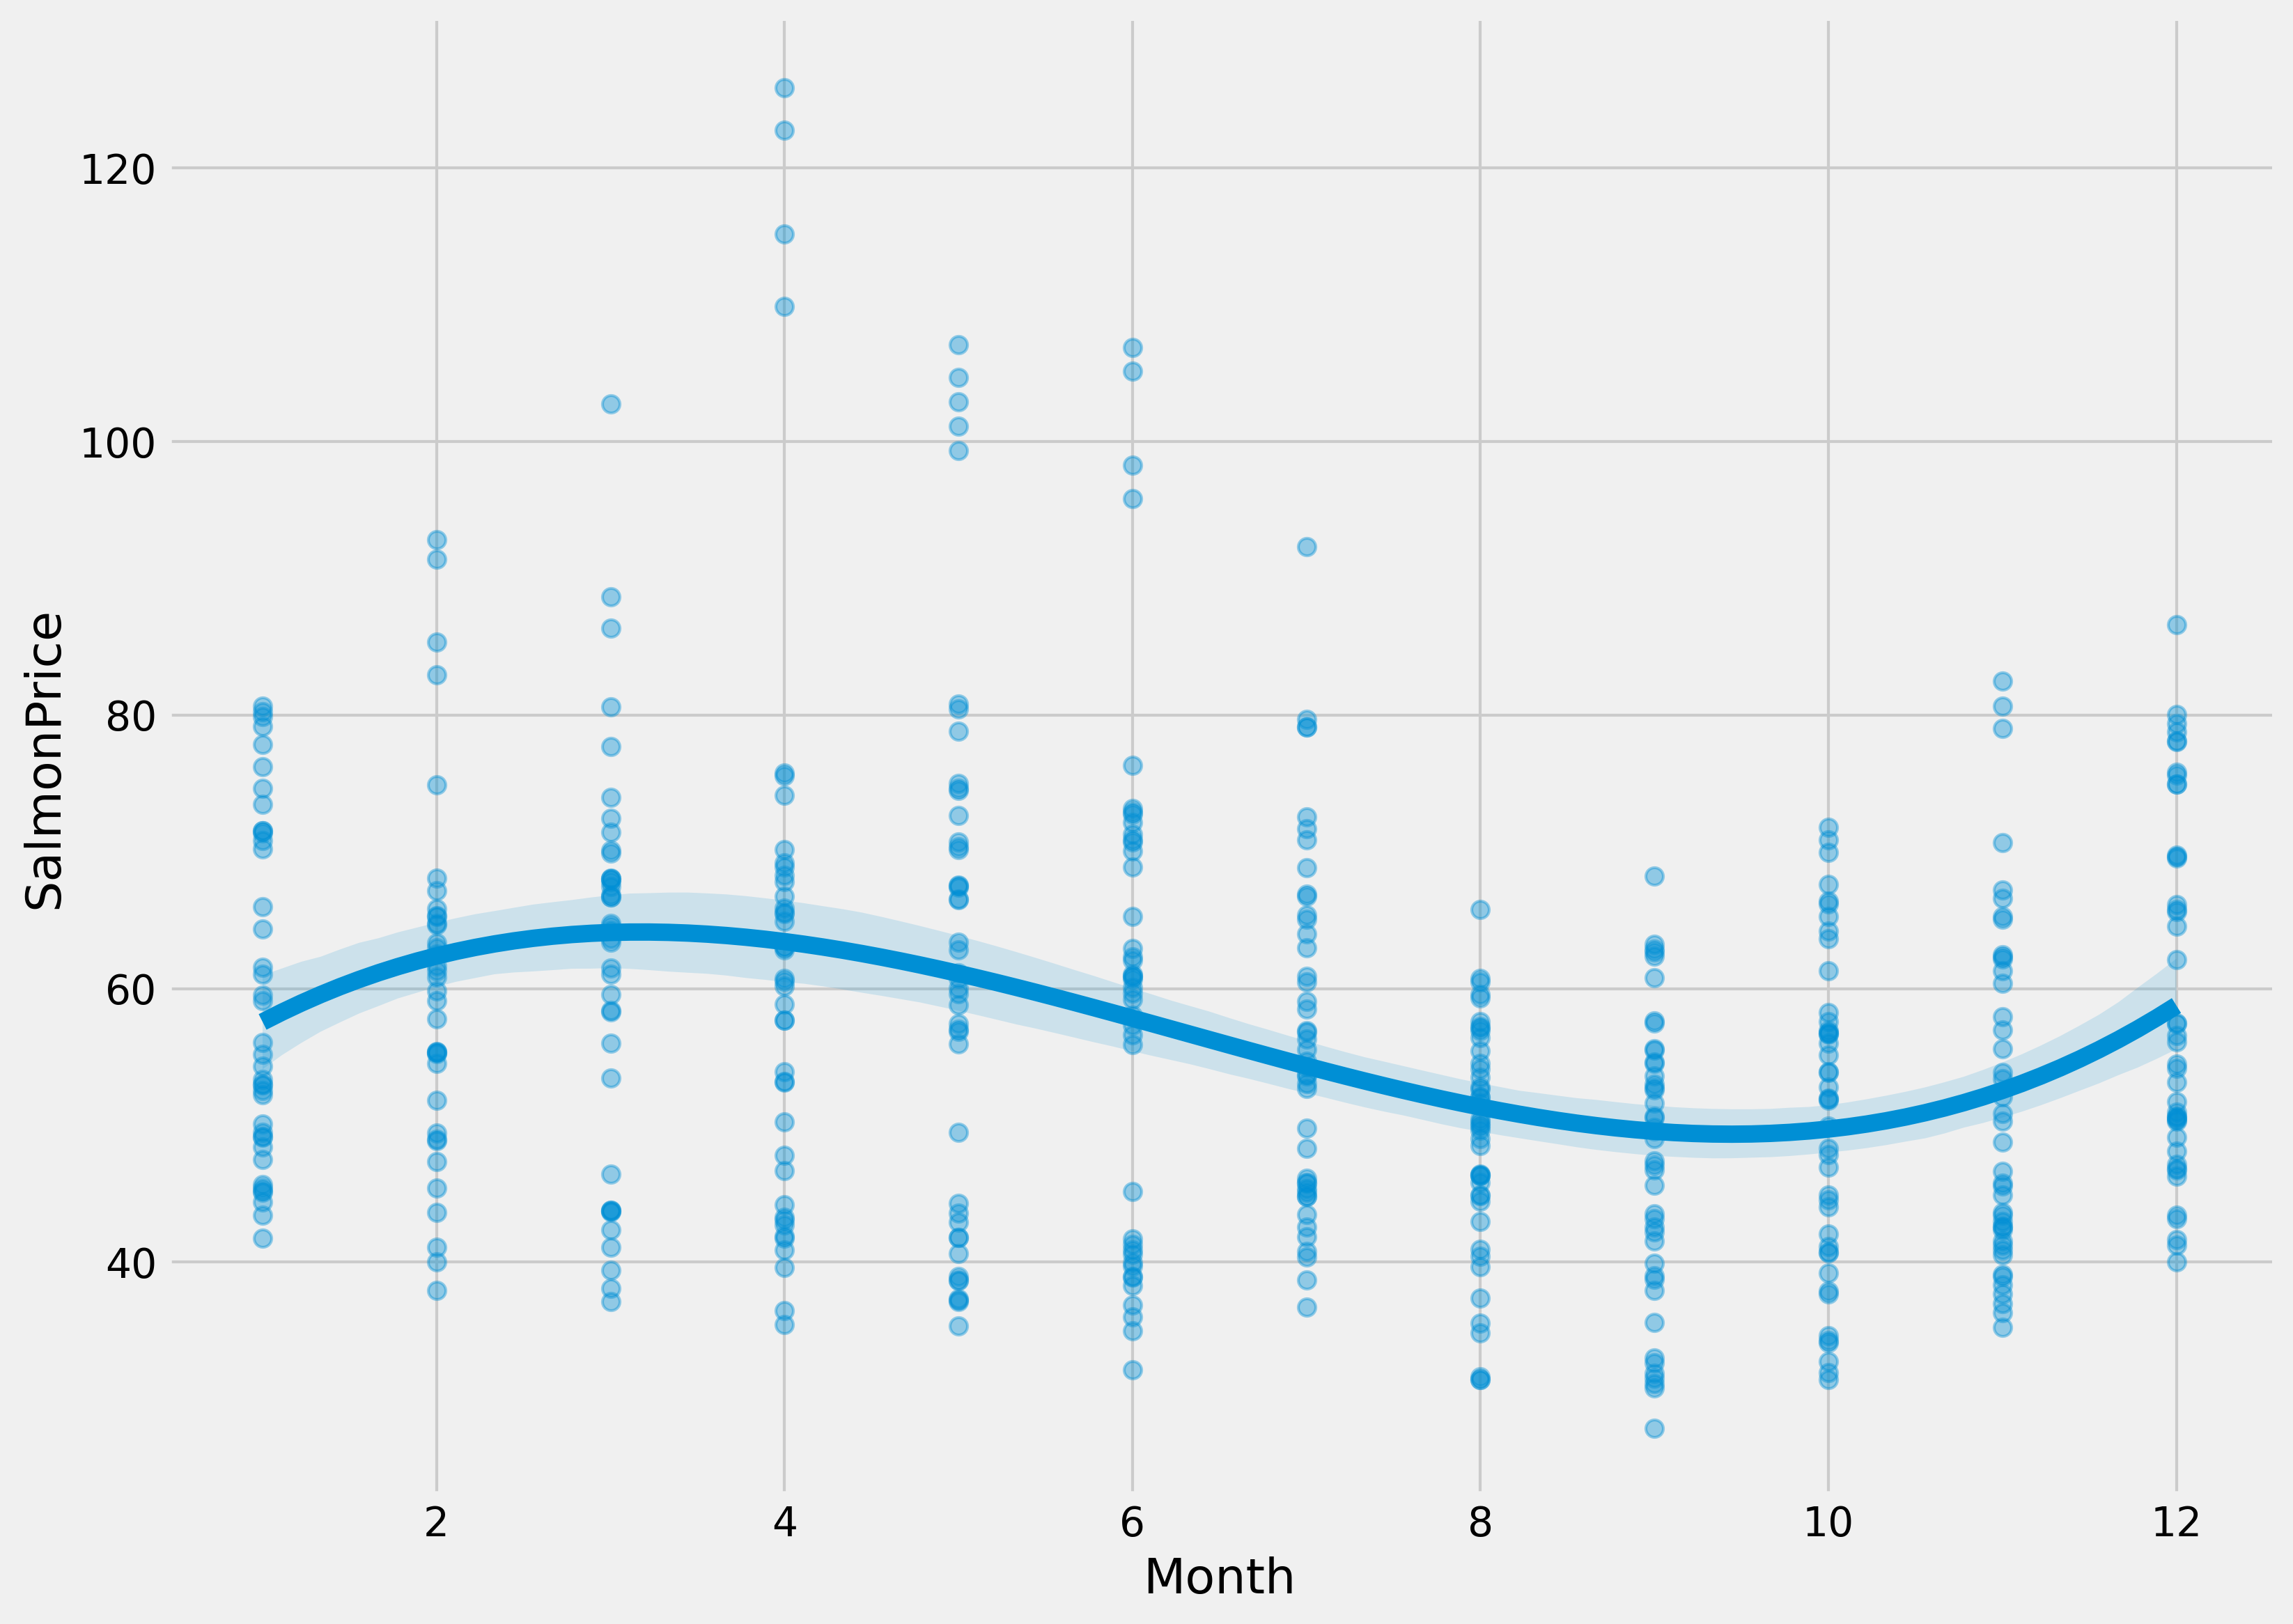
\includegraphics[width=0.8\textwidth]{data/Figures/Descriptive/seasonality.png}
    \caption[Seasonality of the salmon price]{Seasonality of the salmon price}\label{fig:Seasonality of the salmon price}
\end{figure}

We see that there is a clear peak in the price in April. The price level in general is at its highest in the spring and early summer and at its lowest in late summer and early fall. Looking at our regression line we see that this is true for most of the data, and not only the very top price points of each month. This line also visualizes the spread in price for the individual months and we can see that the higher spread in price follows the months of the highest prices. This might not be due to higher prices differences during the spring. This characteristic is at least in part caused by the fact that the rising price level is amplifying the spring prices making the average of the earlier years a lot lower than the average of the later. This in turn makes it look like there are larger price differences during these months than what is actually the case.

\subsubsection{Comparison between the different types of fish}\label{Comparison between the different types of fish}
We would also like to gain a little bit of insight as to how our variables compare to each other. We start by having a look at the price data for the different types of fish considering whether the cod and halibut is comparable to the salmon price.

\begin{table}[H]
    \begin{center}
    \begin{tabular}{lrrr}
        \toprule
        {} &  SalmonPrice &    CodPrice &  HalibutPrice \\
        \midrule
        count &   507.000000 &  507.000000 &    507.000000 \\
        mean  &    56.746134 &   24.553419 &     58.029858 \\
        std   &    15.455462 &    8.096777 &      7.900179 \\
        min   &    27.870000 &   10.275557 &     36.507234 \\
        25\%   &    44.875000 &   20.365239 &     51.971903 \\
        50\%   &    55.460000 &   24.035290 &     59.300626 \\
        75\%   &    65.710000 &   30.478502 &     63.418690 \\
        max   &   125.870000 &   49.076318 &     79.182888 \\
        \bottomrule
    \end{tabular}
    \end{center}
    \caption{Descriptive statistics for the fish price data}
\end{table}

Looking at this we can see that the halibut is very similar to the salmon in price but with a larger minimum and a lower maximum as well as half the standard deviation. In general the halibut price seems to be much more stable. Looking at the cod price we see that its quite a bit lower compared to the two others. Relative to its size it has a lot more similar characteristics to the salmon price in terms of price stability. If we scale it by two, we will see that the mean price becomes 49 compared to the 55 of salmon and the standard deviation becomes 16 compared to the 15,5 of salmon. This indicates that the relative swing in price of cod is of the same magnitude as the swing in price of salmon. However, the salmon price has a lot higher maximum price then the two others even if scaling the cod price by two, this may mean that we have some outliers at the very top of our salmon price range. To confirm this, we will look at a boxplot of the price data.

\begin{figure}[H]
    \centering
    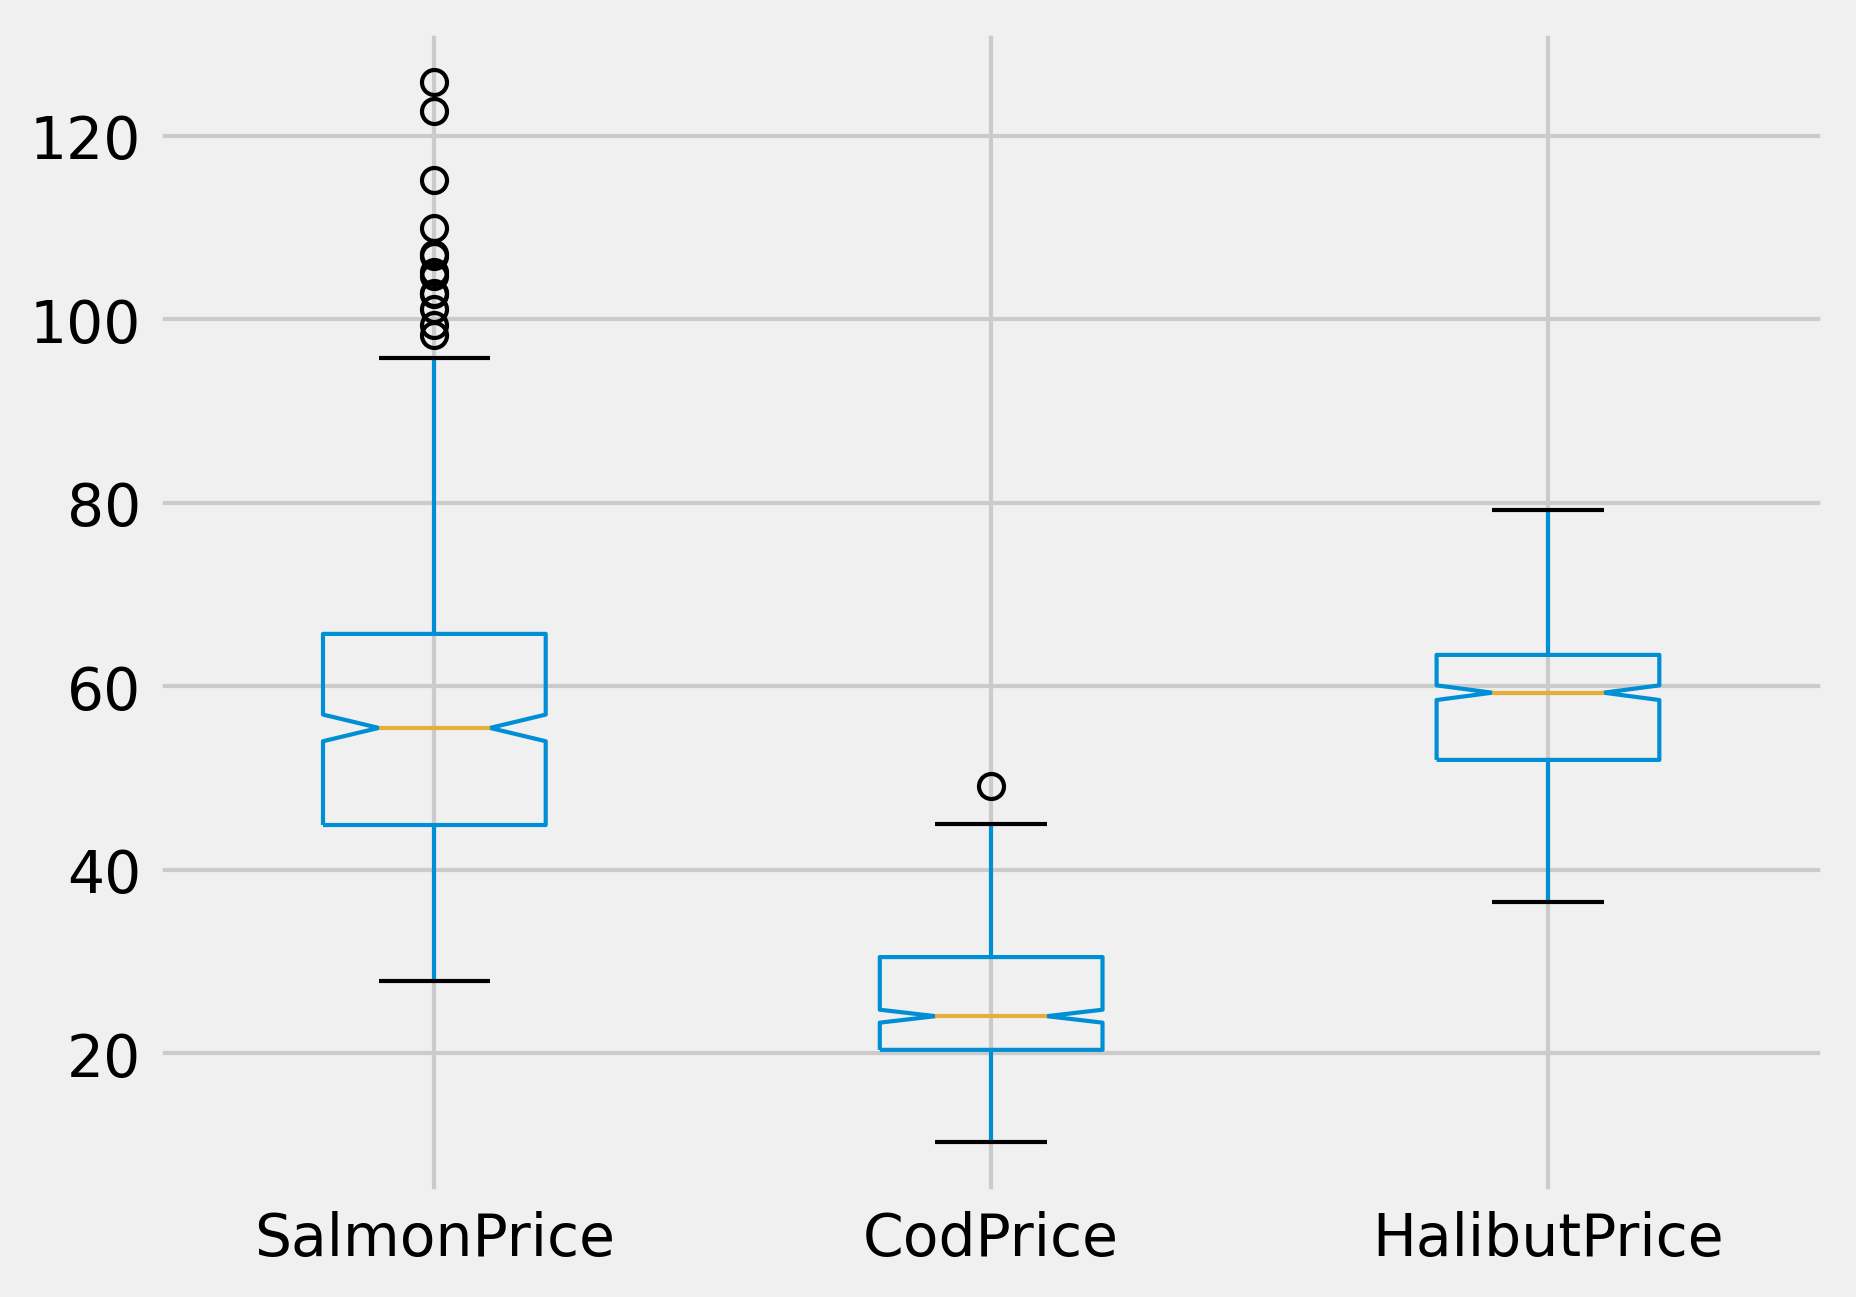
\includegraphics[width=0.8\textwidth]{data/Figures/Descriptive/Whisker.png}
    \caption[Whisker boxplot of fish price data]{Whisker boxplot of fish price data.}\label{fig:Whisker boxplot}
\end{figure}

Looking at the boxplot we can see that the salmon does indeed have a lot of outliers at the top of the price range. The cod price seem to have a singular outlier whilst the halibut price has none. The hight of the boxes also visualises the aforementioned price range differences well. Looking at the yellow lines representing the average. We can see that the cod and halibut have an average situated higher in middle of the 50th percentile. This means that the distribution of these two are a little bit skewed to the right.

\subsubsection{Covariance and correlation}\label{covariance and correlation}
By exploring the covariance and correlation of our chosen variables we aim to uncover if they can be used as indicators for the salmon price. A good covariance between the salmon price and another variable, means that moving that variable would result in a likelihood of the other variable moving accordingly either positively or negatively. If the covariance is high, it is interesting to look at the correlation for the same variables and see if we expect to see a change in the same direction for the corresponding variable. This property is what we are looking to exploit in our predictive models and finding variables that possess this property is key to the accuracy of our predictions.

From the matrices in figures~\ref{fig:CovMatrix} and~\ref{fig:CorrMatrix} we see that all the variables except months have a pretty good covariance all being above 50. The best ones being the CPI and the Cod Price as we suspected earlier. The corresponding correlations of CPI and cod are also the highest correlations to our main variable which means that these two variables are more likely to be good indicators for the salmon price. The other variables have a lower covariance and correlation, but still have a positive covariance which means that they are still good candidates for our predictive models. The months variable has a negative covariance which means that the salmon price is more likely to go down in the winter months. This is a good indicator for the salmon price as we know that the salmon price has a seasonal tendency. Although a month term might not be the best way to capture it.
\newpage
\begin{figure}[H]
    \centering
    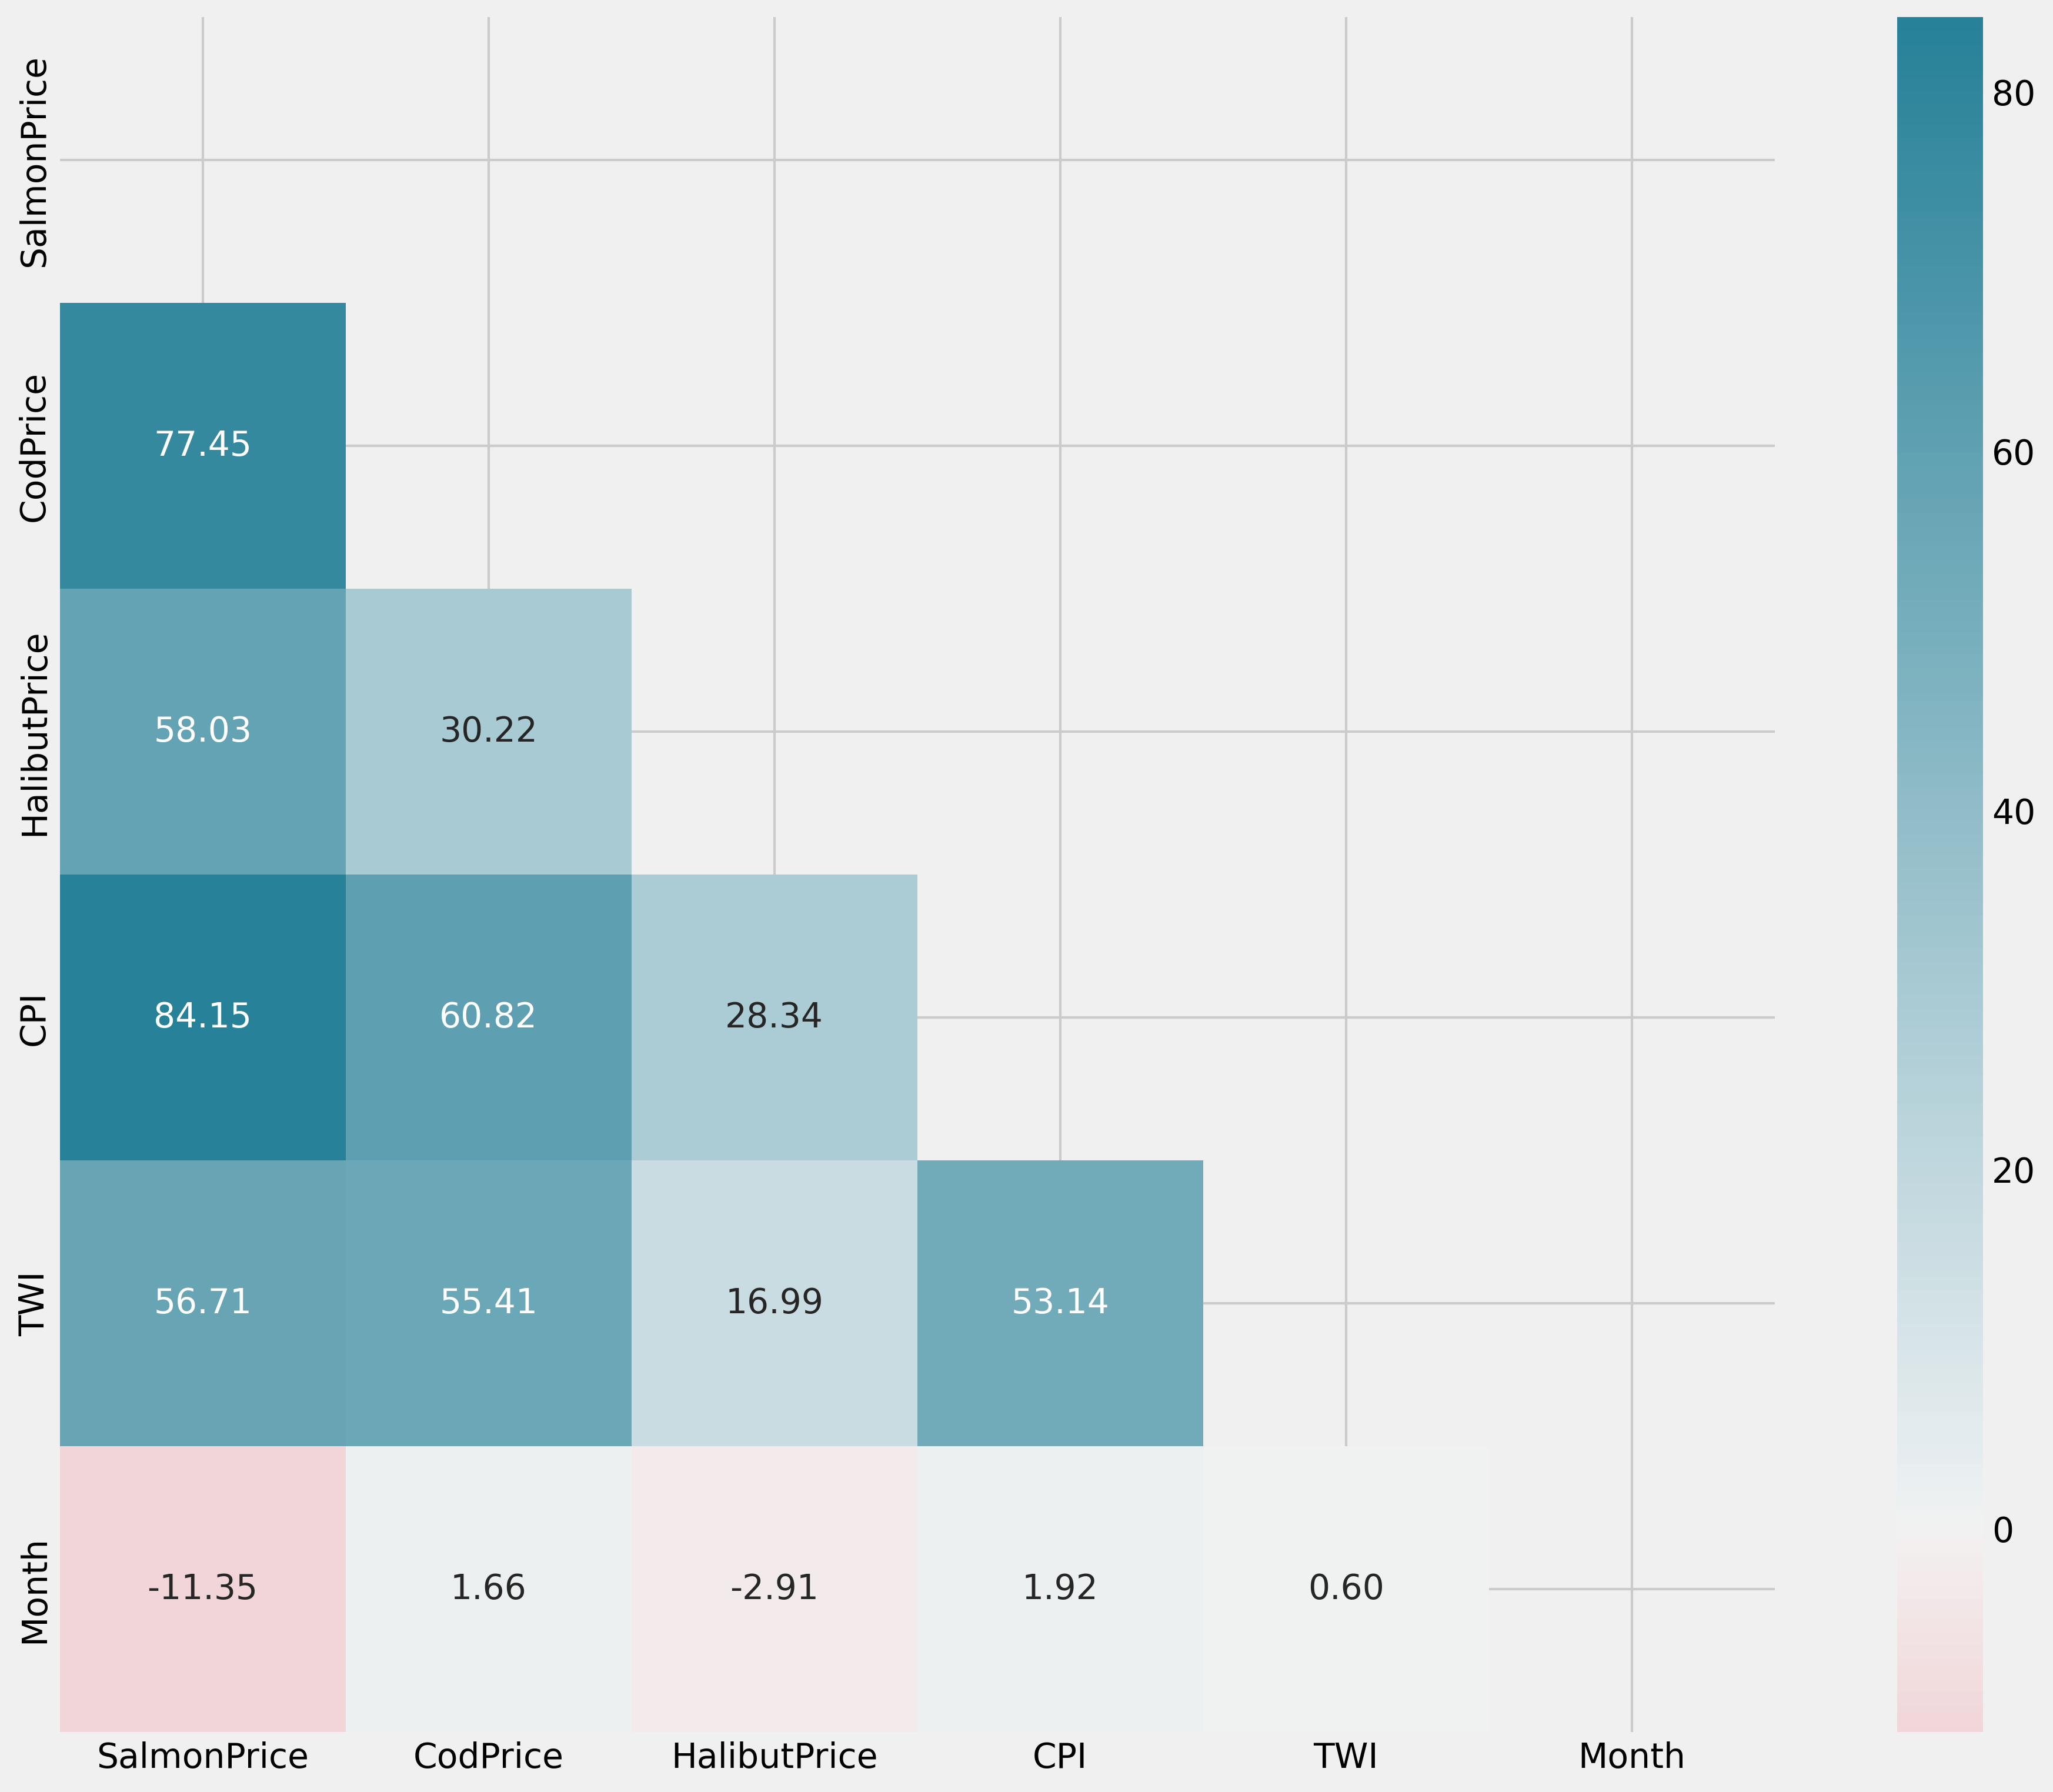
\includegraphics[width=0.8\textwidth]{data/Figures/Descriptive/CovMatrix.png}
    \caption[Covariance matrix]{Covariance matrix with all variables}\label{fig:CovMatrix}
\end{figure}

\begin{figure}[H]
    \centering
    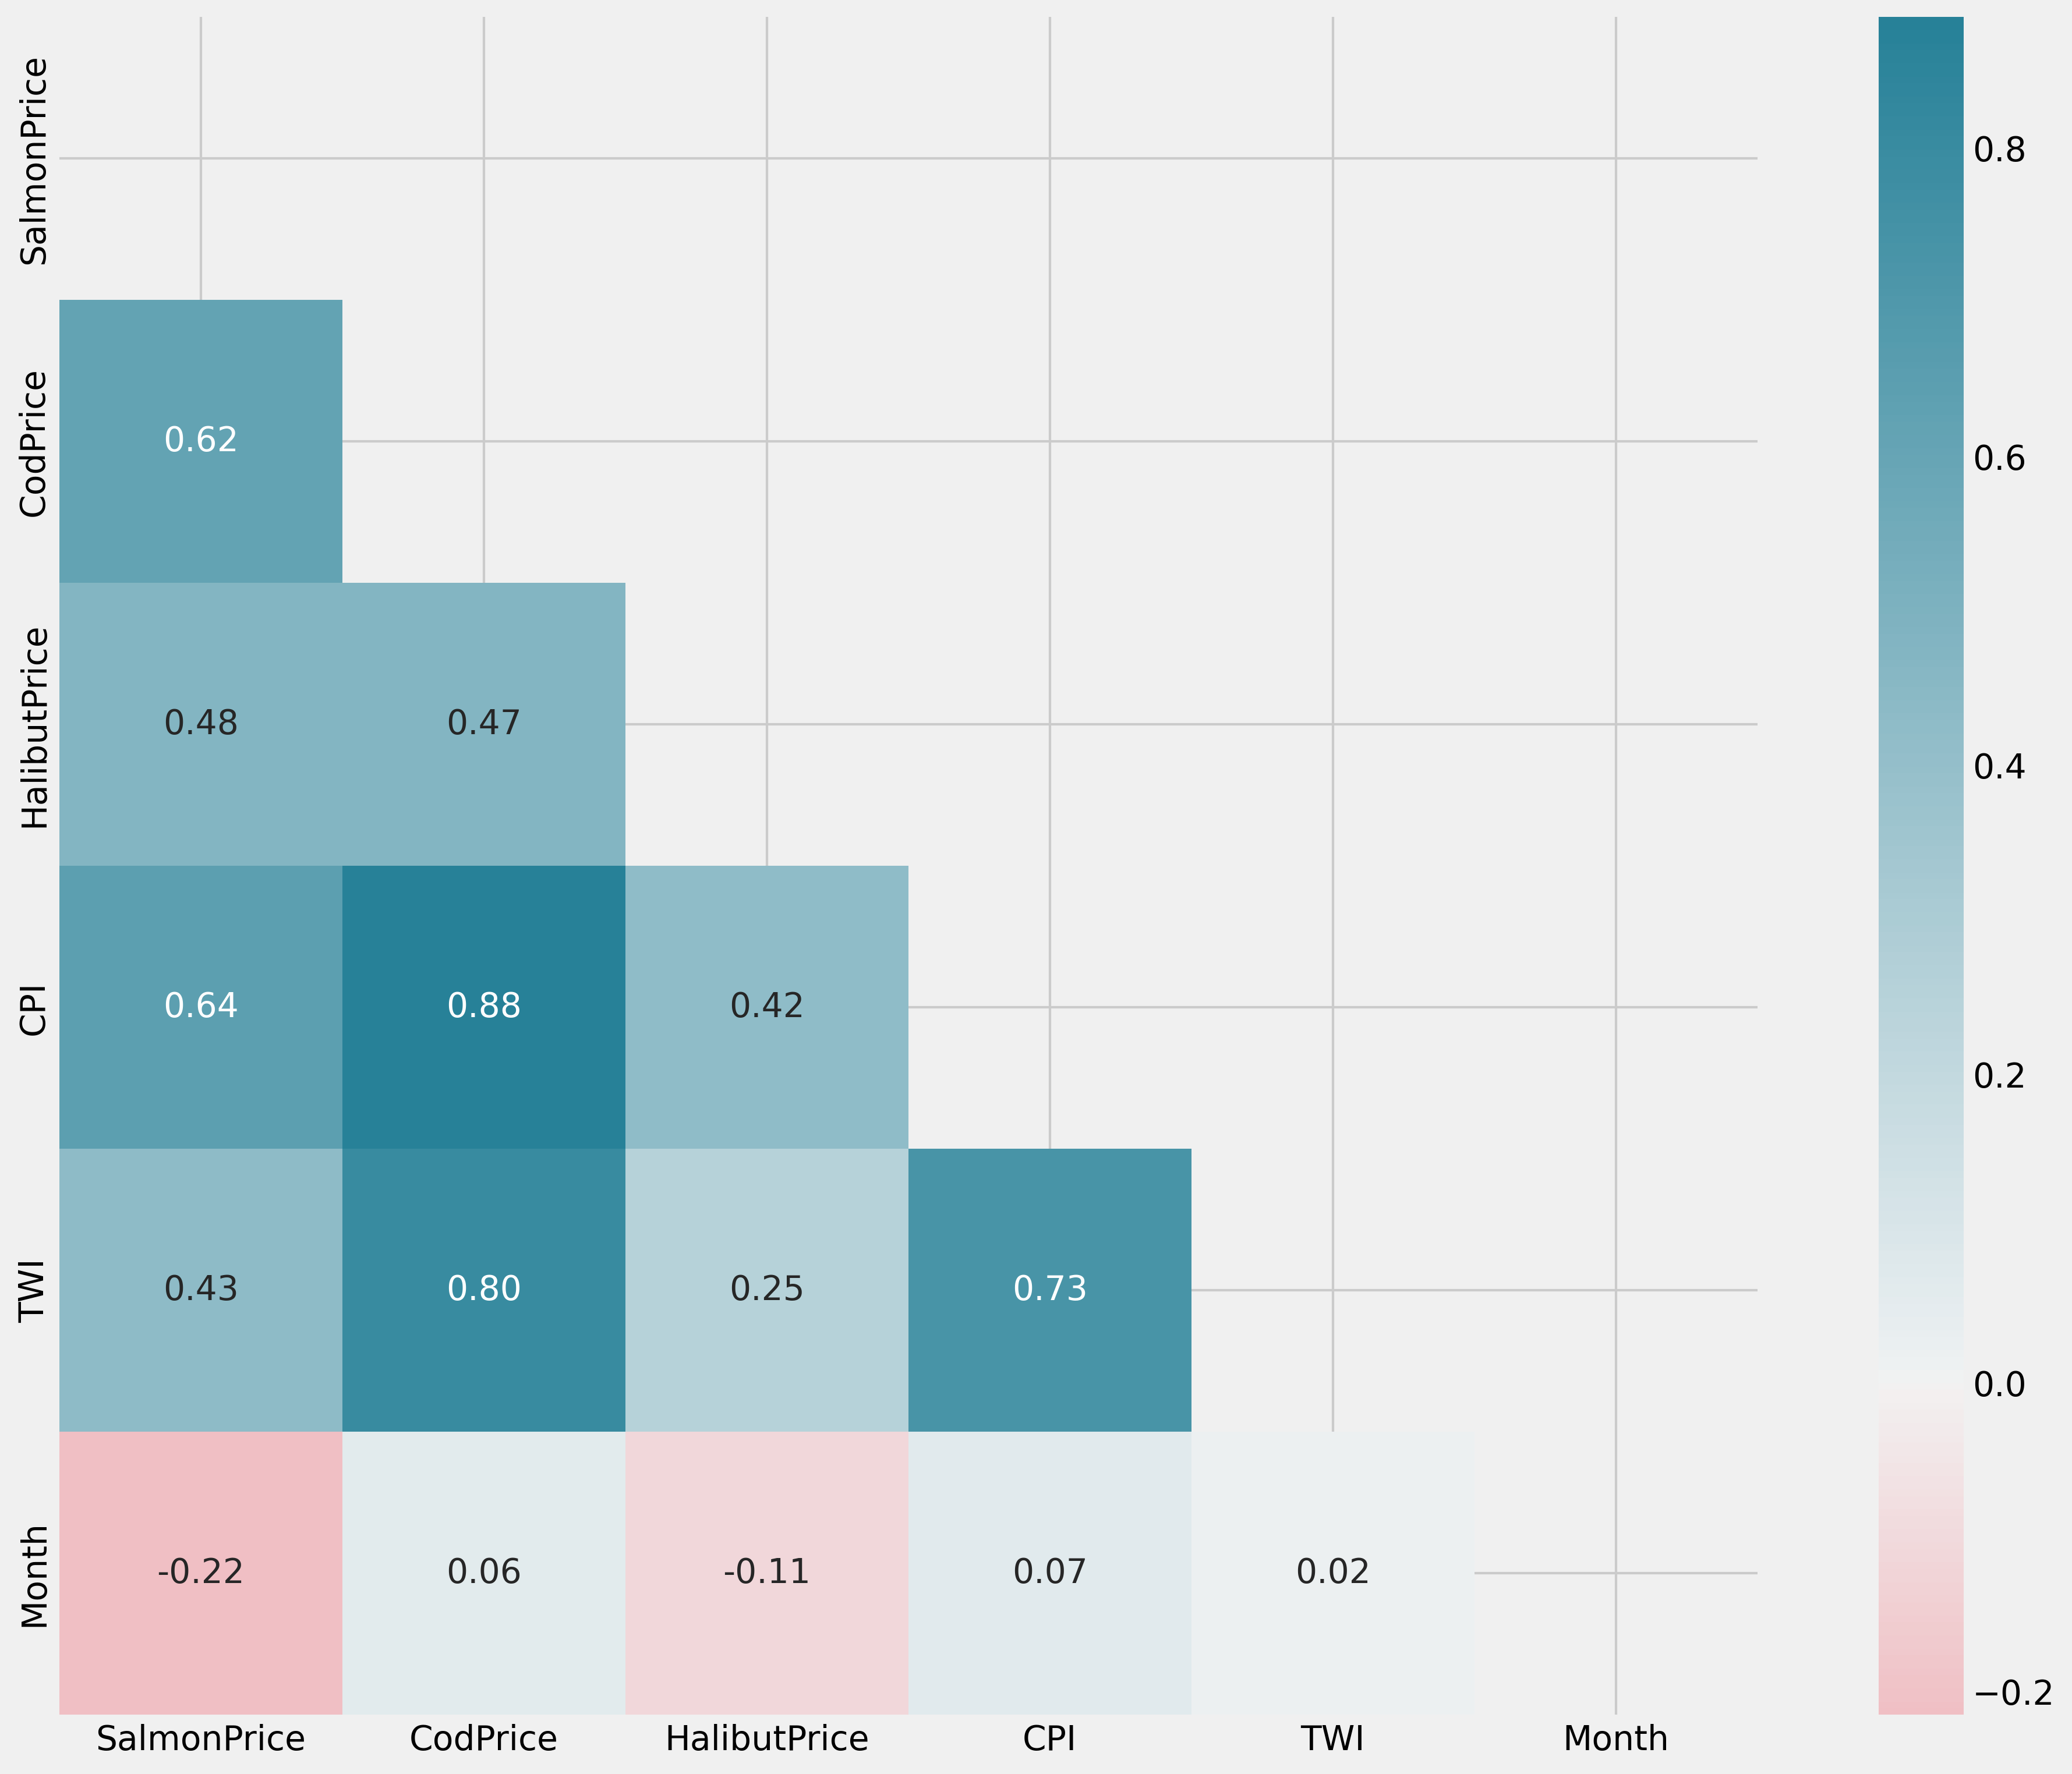
\includegraphics[width=0.8\textwidth]{data/Figures/Descriptive/CorrMatrix.png}
    \caption[Correlation matrix]{Correlation matrix with all variables}\label{fig:CorrMatrix}
\end{figure}

\subsection{Data preprocessing}
In order to use the data for prediction in our models we need to prepare the data. In our case this means to split the data into a training and test set. We will use the same split for all of our models, so that we they are comparable. The test set will be the last year of the data, 2021. The training set will be the rest of the data, 2013--2020. A very important aspect of forecasting using machine learning algorithms is that the test set should be `invisible' throughout the training process, otherwise we might get data leakage and consequently, a false sense of how well the model performs.~\parencite{brownlee_2016}
\subsection{ARIMA and SARIMAX}\label{ARIMA and SARIMAX Methodology}

One important prerequisite for the ARIMA model is that the data is stationary. This can be done either by analysing the time-series itself and noticing the variance and trend, or by using the Augmented Dickey-Fuller test. 
After this is done, the next step will be to find the optimal parameters for the ARIMA model. This is usually done by looking at the ACF and PACF plots. 
When the optimal parameters are found, the model can be fitted and used to predict future values.~\parencite{hyndman_athanasopoulos_2021}

\subsubsection{Determining stationarity}\label{DeterminingStationarity}
The Augmented Dickey-Fuller test is a statistical test that can be used to determine stationarity. The null hypothesis of the test is that the time-series is non-stationary. If the p-value is less than the significance level, the null hypothesis is rejected and the time-series is expected to be stationary.
Using the Augmented Dickey-Fuller test on the Salmon Price data, we get a p-value of 0.02406, this means that we can reject the null hypothesis at a 95\% confidence level according to this test. The data may therefore be stationary.~\parencite{Dickey_Fuller1979}

In order to better understand why the data is not stationary we can plot the data and look at the variance, trend and seasonality. This is done by decomposing the data into its components. We then get the following plot: 

\begin{figure}[H]
    \centering
    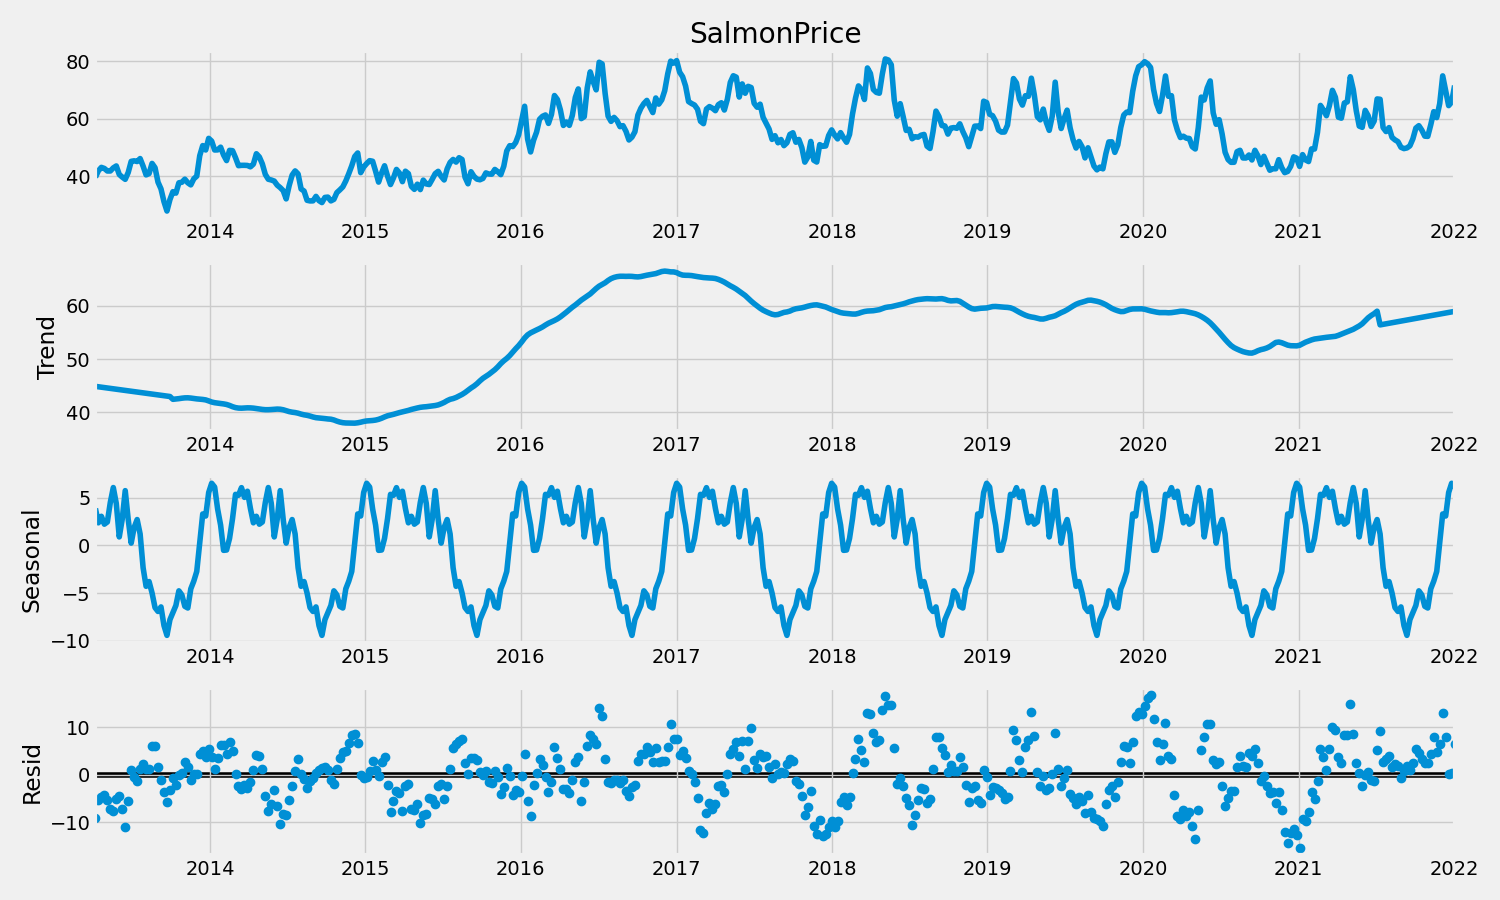
\includegraphics[width=0.8\textwidth]{data/Figures/ARIMA/Decomposition.png}
    \caption[Decomposition of the Salmon Price data]{Decomposition of the Salmon Price data.}\label{fig:Decomposition}
\end{figure}
Examining the decomposed data in Figure~\ref{fig:Decomposition} there are especially two things that stand out. The first is the trend, which is clearly increasing. The second is the seasonality. There is a clear yearly seasonal trend where the price is higher in the summer months before decreasing during the autumn and reaching a low in the winter. From this we draw a different conclusion than the Augmented Dickey-Fuller test. According to the plot, the data is not stationary and needs differencing. In the ARIMA model, this will be done by setting $d$ to 1 or more. 

The exact number of differencing needed can be found either by using the ADF-test on the differenced data and looking for when the p-value is less than the critical value, or by looking at the autocorrelation plot and using rules set out by \textcite{nau_2019} to determine the number of differencing needed. 
\begin{figure}[H]
    \centering
    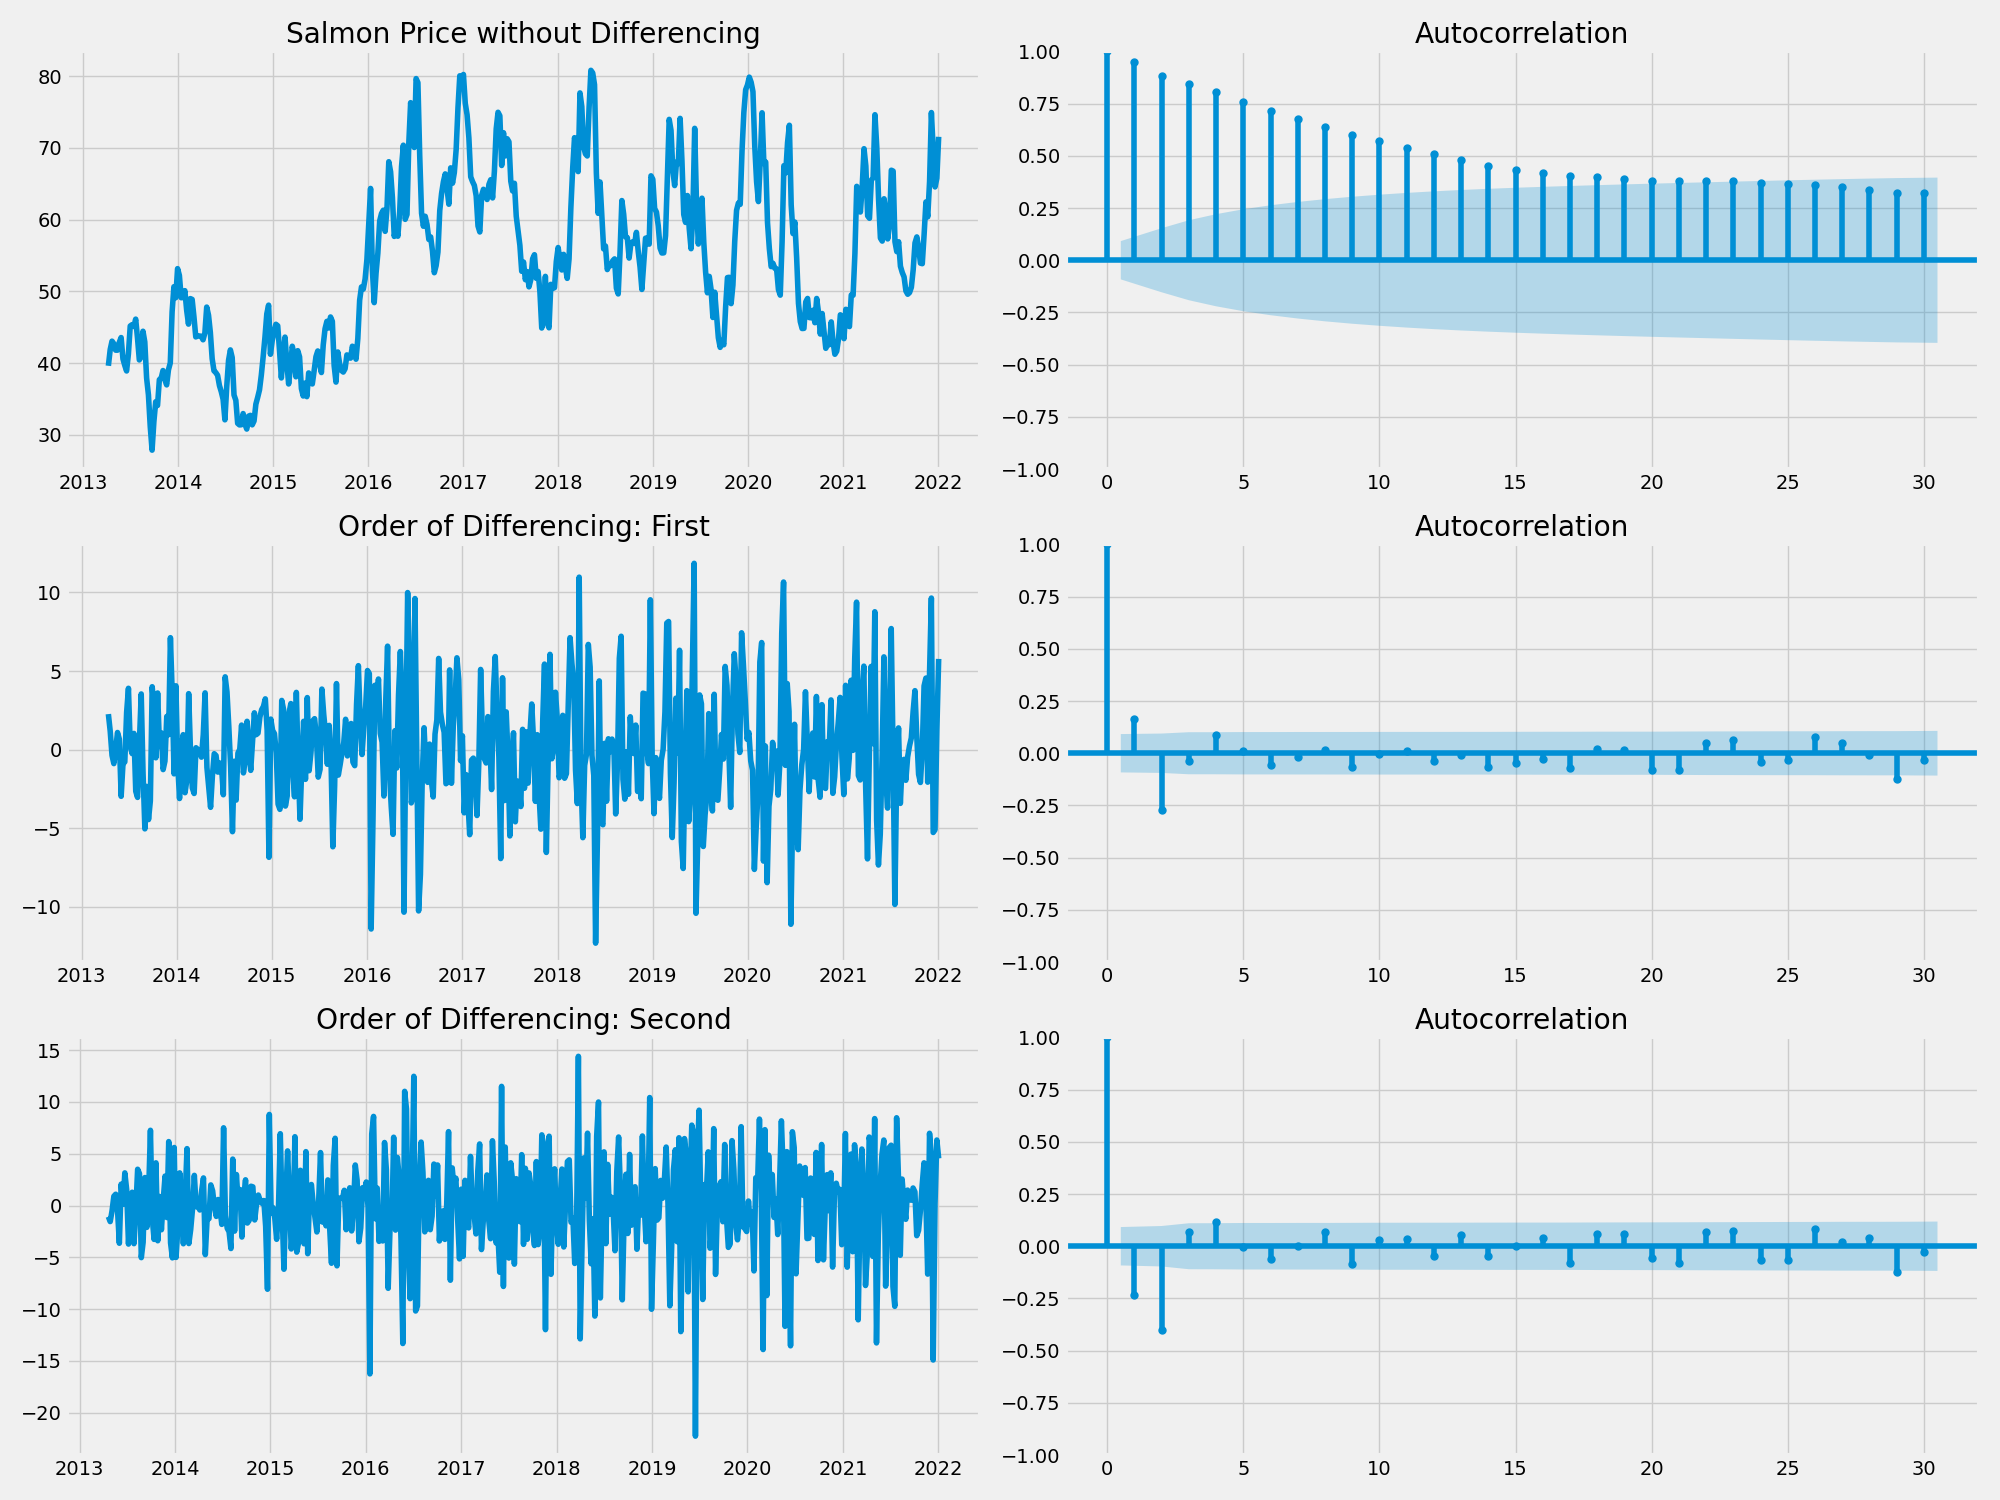
\includegraphics[width=0.8\textwidth]{data/Figures/ARIMA/Diff1_ACF_30.png}
    \caption[Different orders of differencing]{Different orders of differencing.}\label{fig:ACF_Differencing}
\end{figure}
Examining the trend and autocorrelation in Figure~\ref{fig:ACF_Differencing} we can see that the original data without differencing has both a clear trend and a slow decay in the autocorrelation plot with a high number of positive lags. Following the first rule from \textcite{nau_2019} we can conclude that the data needs at least one order of differencing.

After just a single order of differencing, the trends start to flatten out and fluctuate around 0. The autocorrelation plot also drops sharply after the first lag, and is then quite small and patternless, this follows the second rule from \textcite{nau_2019} and will often be a sign that higher differencing is not needed. Running the Augmented Dickey-Fuller test on the differenced data, we get a p-value of 3.86388e-24, much lower than the critical value of 0.05. We can therefore reject the null hypothesis and conclude that the differenced data is stationary. 

With a second order of differencing, the trend seems to flatten even more, and the autocorrelation plot shows a sharp negative decline for the first and second lag, this may be a sign that the data is over-differenced. This is not optimal as over-differencing will lead to a loss of historical information and trends. It is therefore of utmost importance to find the order of differencing that both makes the data stationary and keeps the historical memory intact. Over-differencing is a common mistake when fitting non-stationary data to machine learning models, and can lead to the model not being able to capture the underlying trend.~\parencite{lopezde_prado2018}

A third way to determine the optimal number of differencing is, according to \textcite{nau_2019}, to look at the standard deviation of the plot at different orders of differencing. Following his rule number 3, the optimal number of differencing is the one where the standard deviation of the plot is the lowest. Examining Table~\ref{StdDevTable} we can see that the standard deviation of the data is lowest at the first order of differencing. After this the standard deviation increases, and there is no reason to believe any higher number of differencing will reduce the standard deviation. 

\begin{table}[H]
    \begin{center}
        \import{data/Figures/ARIMA/}{StdDevTable}
        \caption{\label{StdDevTable}Standard deviation of the differenced data.}
    \end{center}
\end{table}

We can therefore conclude that the optimal number of differencing should be either 0 or 1.

\subsubsection{Autoregression and Moving Average}
The next step in a regular ARIMA model is to identify the optimal AR and MA terms needed to fit the model. This can be done by comparing different models by looking at the AIC and BIC values, but with larger models this would constitute an unnecessary use of computational power. A more efficient way to find the optimal terms is to look at the ACF and PACF plots of the data and use the rules set out by \textcite{nau_2019} to determine the optimal $p$ and $q$. 
\begin{figure}[H]
    \centering
    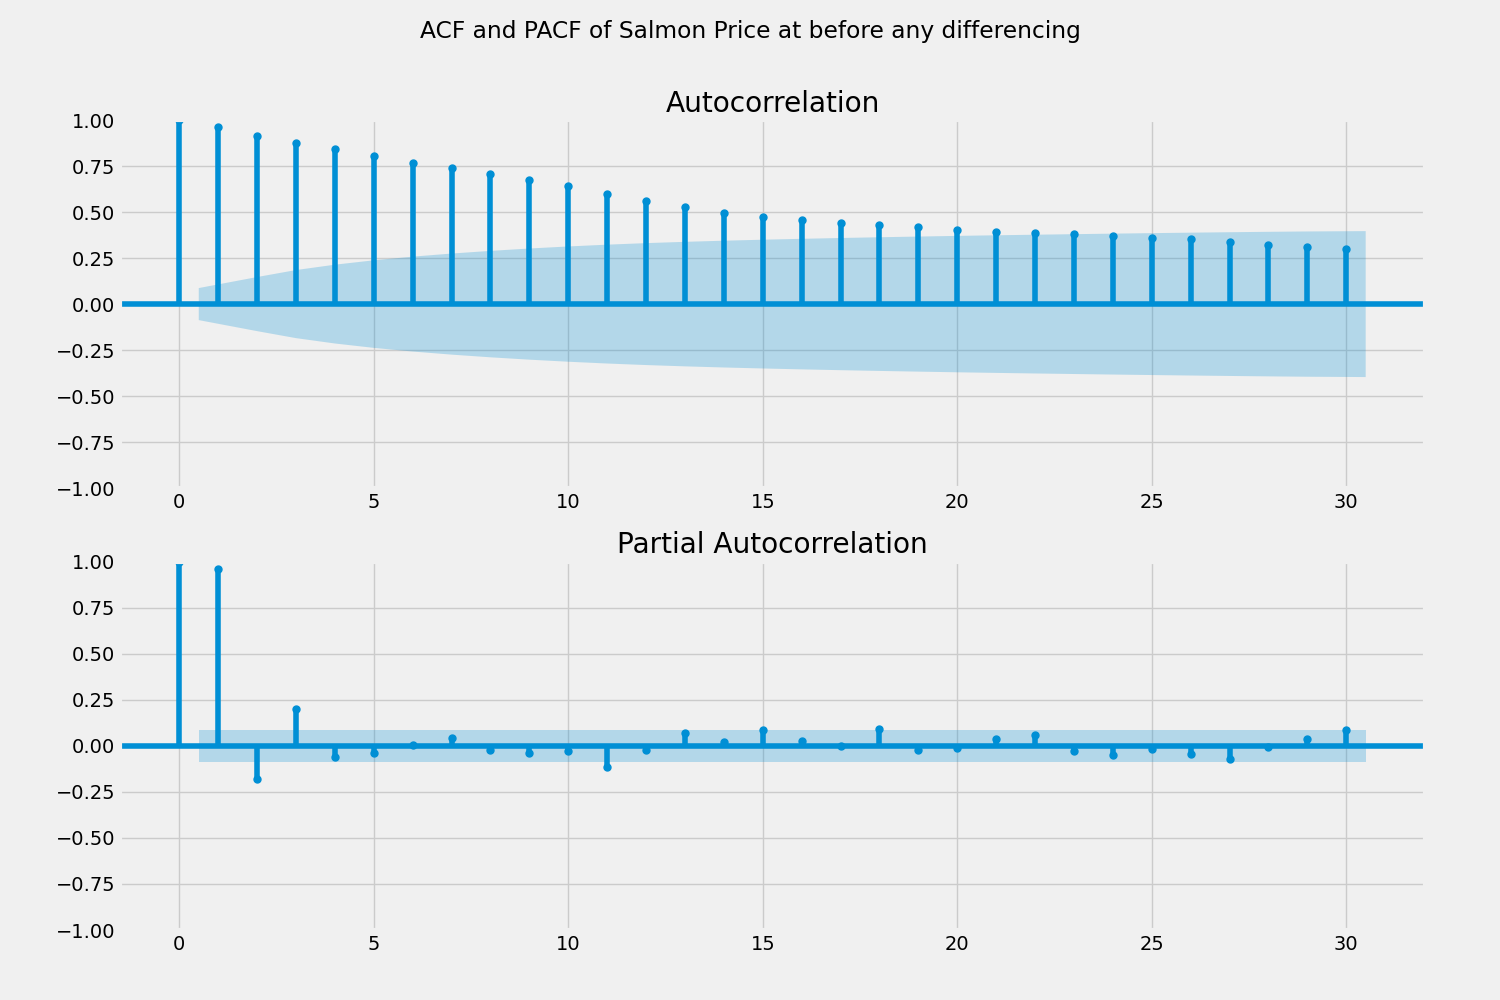
\includegraphics[width=0.8\textwidth]{data/Figures/ARIMA/OrigACF-PACF_30.png}
    \caption[ACF and PACF plots of Salmon price]{ACF and PACF plots of Salmon price.}\label{fig:Orig_ACF_PACF}
\end{figure}

The most noticeable part of the ACF plot in Figure~\ref{fig:Orig_ACF_PACF} is the slow decline of the autocorrelation after the first lag. This is a sign that the data is not white noise, and that there is a correlation between the data and its lags. According to \textcite{nau_2019}, this is called an `AR signature' and is a clear sign that we need to add an AR term to the model, rather than adding an MA term. To find the optimal amount of AR terms needed we can look at the PACF plot. As a rule of thumb, the optimal number is where the PACF plot exhibits a clear drop. In Figure~\ref{fig:Orig_ACF_PACF} we can see that the PACF plot drops sharply after the lag 1, and then fluctuates around 0, mostly within the confidence interval. Therefore, without any differencing, the optimal number of AR terms is 1. But, as we concluded in~\ref{DeterminingStationarity}, the data needs at least one order of differencing. We therefore need to look at the ACF and PACF plots of the differenced data.
\begin{figure}[H]
    \centering
    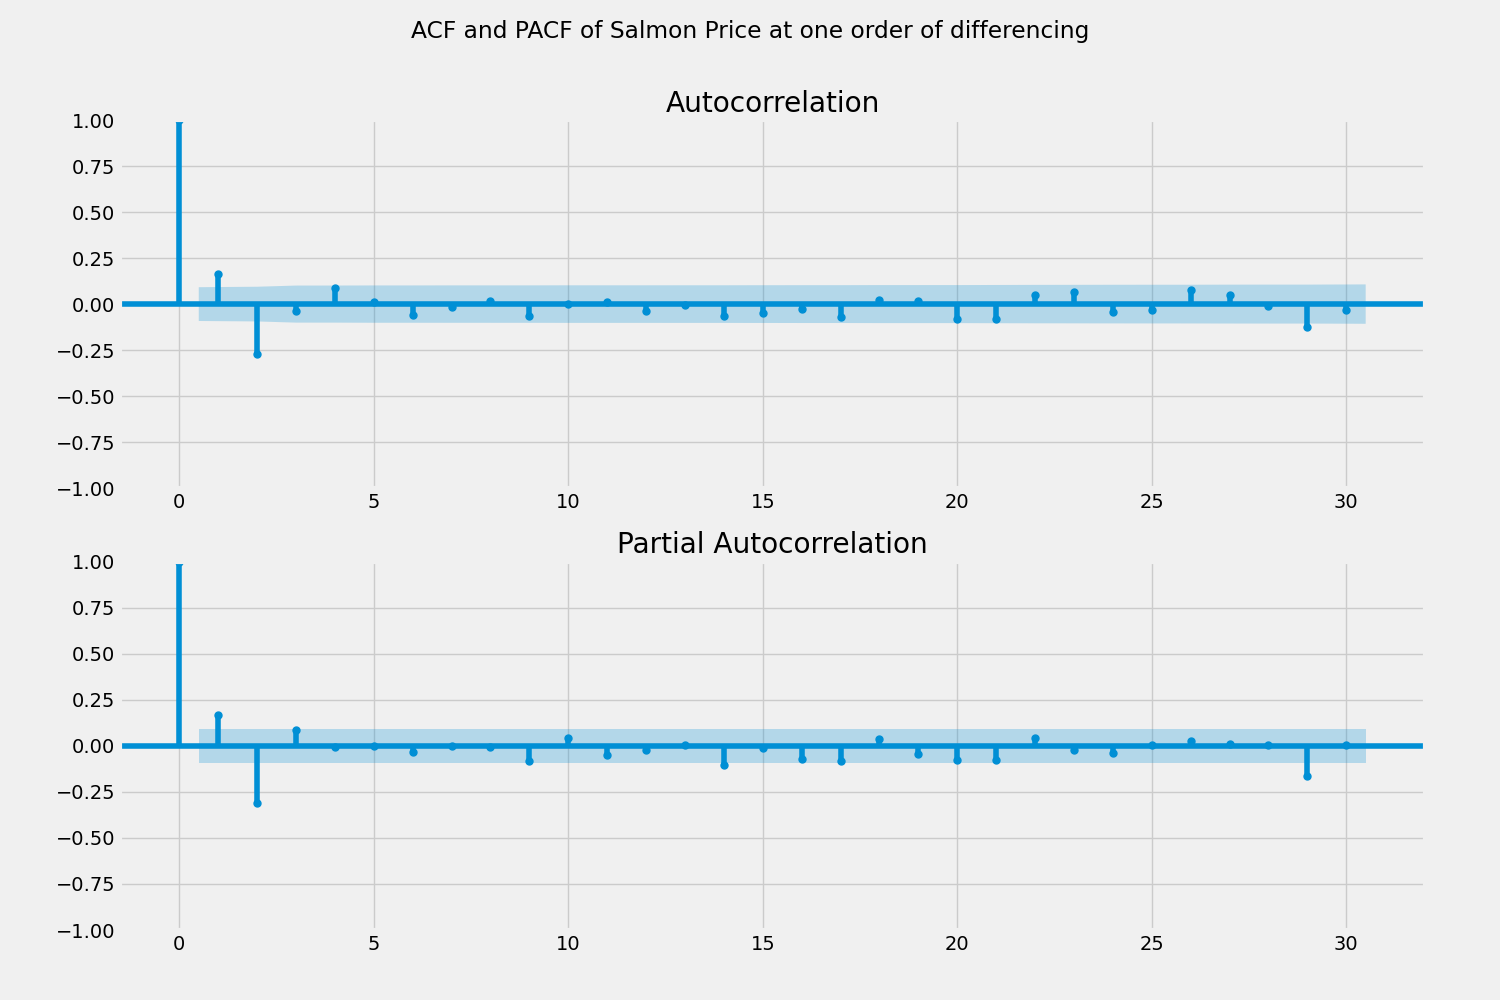
\includegraphics[width=0.8\textwidth]{data/Figures/ARIMA/DiffACF-PACF_30.png}
    \caption[ACF and PACF plots of differenced Salmon price]{ACF and PACF plots of differenced Salmon price.}\label{fig:Diff1_ACF_PACF}
\end{figure}

Examining the ACF plot in Figure~\ref{fig:Diff1_ACF_PACF} we can see that the autocorrelation now has a much more rapid decline compared to the original data. The PACF plot exhibits some of the same characteristics as the original data, but with a much sharper decline for the first lag. Nevertheless, as the first lag of both the ACF and PACF plot is positive and significant outside the 95\% confidence interval, there should be at least one AR term. At the same time, there is also some negative lags in both the ACF and PACF plots which may indicate that there should be an MA term, but according to \textcite{nau_2019}, we should be careful mixing AR and MA terms in ARIMA models, as they may cancel each other out. The best model will, in most cases, consist solely of either AR or MA terms.

As the interpretation of visual plots and clues from these can be a bit subjective, we should employ some objective test to determine the optimal number of $p$ and $q$. The most straight forward way to do this is to perform an iterative search over the possible values of $p$ and $q$ and then compare the AIC and BIC values of the different models, as well as comparing the mean squared error of the predictions from the models.  

\subsubsection{Seasonality}
Hitherto we have only considered the non-seasonal ARIMA model, but as with many time series, the Salmon price might also exhibit some seasonal patterns and trends. It may therefore be better to add a seasonal part to the model and consequently call it a SARIMA model. One way to determine this is to look at the seasonal part of the decomposed data. The decomposed data shows us what part of the variation in the data is due to the trend, the seasonal part, and the residual part.
\begin{figure}[H]
    \centering
    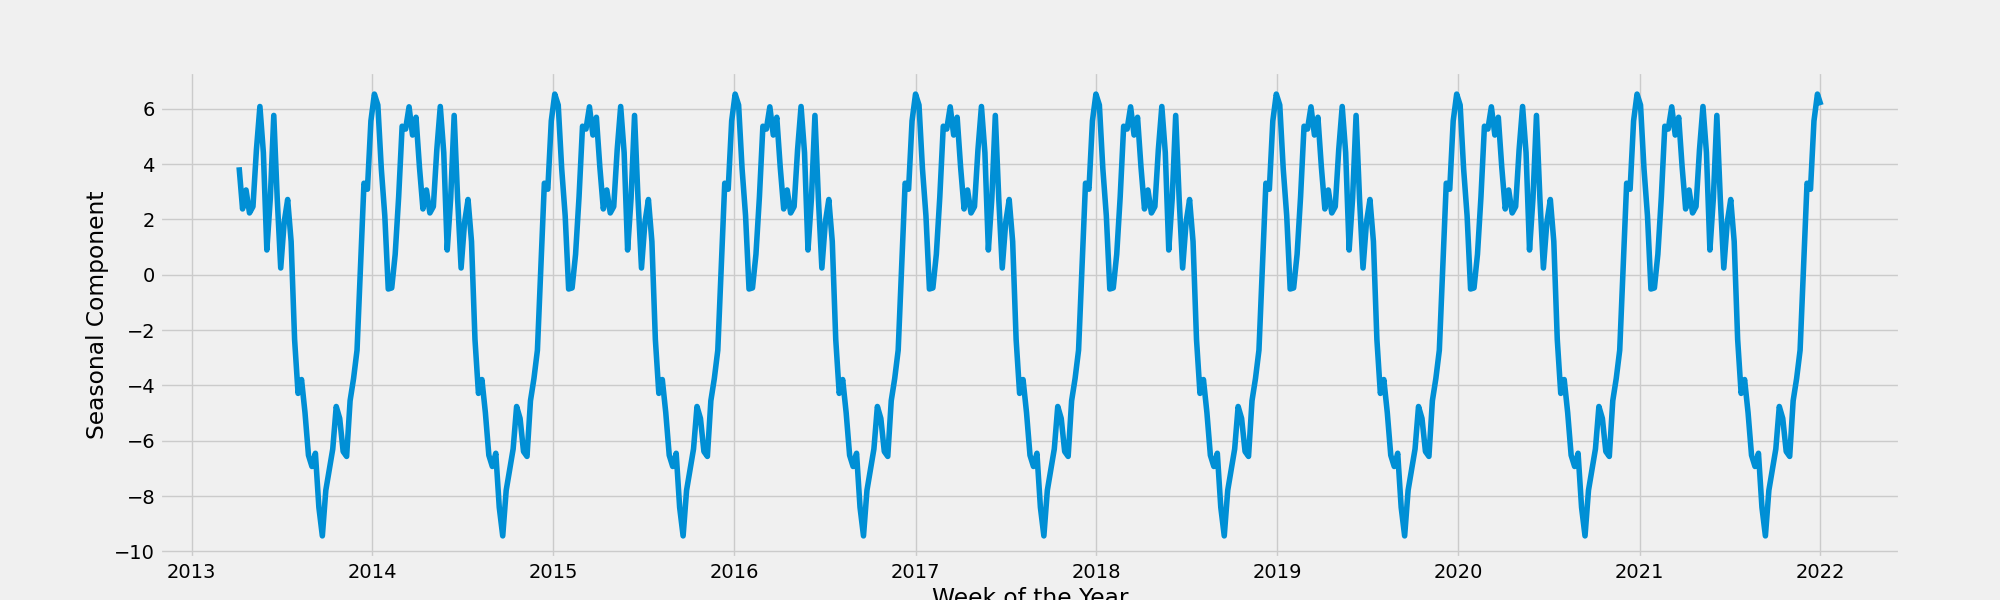
\includegraphics[width=0.8\textwidth]{data/Figures/ARIMA/SeasonalDecompose.png}
    \caption[Seasonal part of the decomposed data]{Seasonal part of the decomposed data}\label{fig:SeasonalDecompose}
\end{figure}

Examining Figure~\ref{fig:SeasonalDecompose} we can see a clear seasonal trend which seems to be repeating itself every 12 months. This could indicate that we should add a seasonal part to the model. As the data is recorded weekly, the $s$ should be 52. \textcite{hyndman_athanasopoulos_2021} mentions that working with weekly data can prove difficult for the ARIMA model to handle as there are, on average, 52.18 weeks in a year, which is not an integer. Nevertheless, we will try to fit a SARIMA model with $s=52$ and compare the AIC and mean squared error of the predictions to the non-seasonal ARIMA model. 

The seasonal part of the ARIMA model also contains $PDQ$ which corresponds to the $pdq$ in the non-seasonal ARIMA model in that they describe the number of seasonal autoregressive terms, the number of seasonal differences, and the number of seasonal moving average terms. In order to determine these terms, we can use the same method as we did for the non-seasonal ARIMA model, namely examine the ACF and PACF plots, but this time for the seasonally differenced data. We can also perform a grid search for the different combinations of AR and MA terms, and in that way obtain the optimal model.

\subsubsection{Exogenous Variables}
One last way to expand on the ARIMA model in order to make it more accurate is to include one or more exogenous variables. This is especially useful if there is some external data that might affect the time series. In our case we suspected that the price of Salmon might be affected by the price of other seafood, as well as the Norwegian Krone. We therefore decided to add these to our dataset and see if it would improve the accuracy of the model.

In order to measure the accuracy of these exogenous variables, we can follow the same procedure as before and compare both the AIC of different models as well as the root mean squared error of the predictions. Comparing the RMSE will probably prove to be a more accurate way of examining the accuracy of the models as AIC cannot handle different levels of differencing and will not work well to compare ARIMA with Tensorflow.~\parencite{brownlee_2017}
\subsection{LSTM --- Tensorflow}\label{Tensorflow_Methodology}
In order to apply the data to a LSTM model, we need to define the different parameters of the model. As a LSTM model consists of an input layer, a hidden layer, and an output layer, we need to define the number of neurons in each layer. And as can be seen in Figure~\ref{fig:Layers}, all neurons between the layers has to be connected, which makes the complexity of the model grow exponentially. Therefore, we need to be careful not to make the model too complex, as it will use too much unnecessary computing power, as well as increasing the risk of overfitting.

\begin{figure}[H]
    \centering
    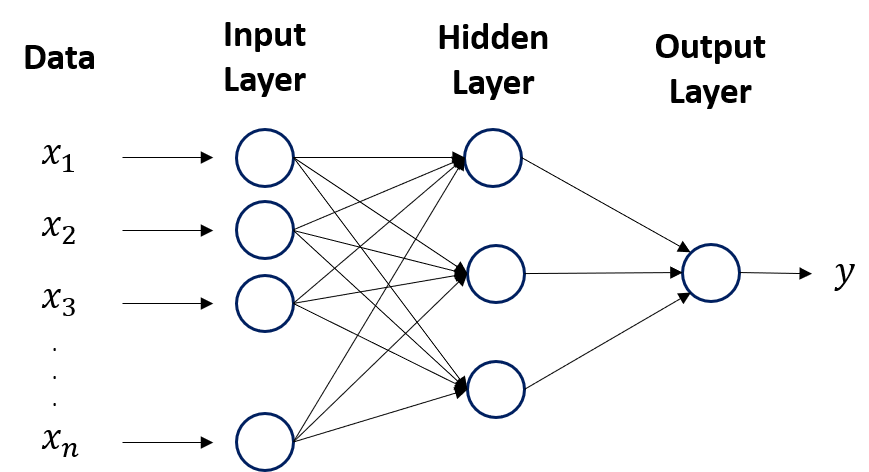
\includegraphics[width=0.8\textwidth]{data/Figures/Neural networks/Layers_lstm.png}
    \caption[Example of the different layers in an LSTM model.]{Example of the different layers in an LSTM model.~\cite{towardsai_2020_1}.}\label{fig:Layers}
\end{figure}

\subsubsection{The input layer}
The input layer is the first layer in the model, and as the name suggests, it is where the input data is fed into the model. The number of input nodes corresponds to the number of features in our model. Therefore, it will depend on the number of exogenous variables we choose to include in the model. We can, for example, choose to only train the model on the previous price of Salmon, and have only one input neuron, or we can include such variables as the price of other seafood and the Norwegian Krone, and have three input neurons. 

In order to prepare the data we will need to scale it between 0 and 1, technically this is not necessary for the LSTM model to work, but it will make the training process both faster and more accurate.~\parencite{brownlee_2019} Secondly, for time series data, it can be helpful to reshape the data into several timesteps, for example, we can use the previous 10 weeks of data to predict the next week. This is expected to make the model more accurate, as it will be able to learn the patterns in the data more efficiently. The reshaped data will be a 3-dimensional array, where the first dimension is the number of samples, the second dimension is the number of timesteps, and the third dimension is the number of features. In mathematics, this sort of array is called a tensor; hence the name Tensorflow.~\parencite{tensorflow_tensors_2023}
\begin{figure}[H]
    \centering
    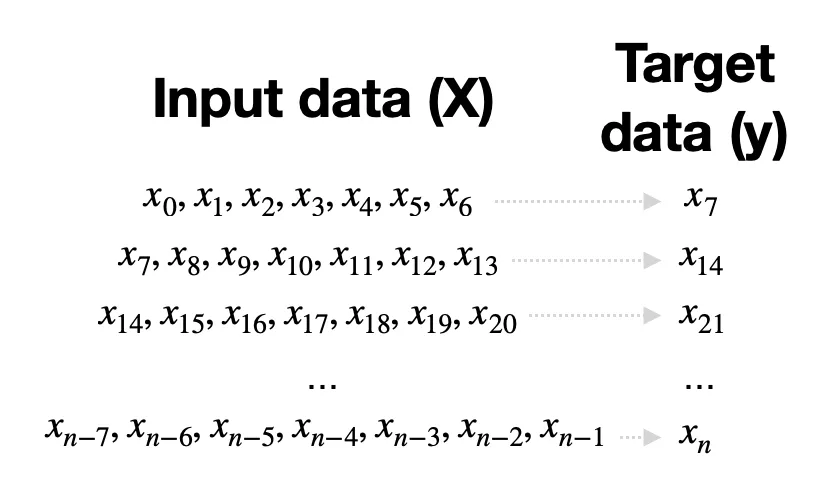
\includegraphics[width=0.7\textwidth]{data/Figures/Neural networks/Sequential_data.png}
    \caption[Example of sequential data in timesteps.]{Example of sequential data in timesteps.~\cite{dobilas_2022}.}\label{fig:Sequential_data}
\end{figure}

\subsubsection{The hidden layer}
The hidden layer is the layer in the model that is responsible for the actual learning, and while the input layer is quite straightforward as the only variables are the number of timesteps and features, the hidden layer is more complicated. This layer consists primarily of multiple interconnected neurons, these neurons can themselves be arranged in layers and result in several hidden layers. The neurons are assigned weights and biases which are used to calculate the output, the weights are used to determine the importance of the input while biases are used to regulate at what point the weight should be added to the output. The weights and biases are updated during the training process in order to make the model as accurate as possible, it achieves this by reducing the loss function, such as mean squared error. In addition to specifying the number of neurons in the hidden layer, we also need to specify the activation function, which is used to determine when the neuron should be activated. The most common activation functions are the sigmoid function, the hyperbolic tangent function, and the rectified linear unit function.~\parencite{sharma_2019}

Consequently, there are a great number of hyperparameters that needs to be chosen before the model can be fitted, and while the goal is to find the optimal model, we also need to avoid overfitting. One way to achieve this is to solely experiment with different hyperparameters and see which combination gives the best results, but this can be a time-consuming process. A more efficient way is to utilize grid search, similarly to the ARIMA model, which will test for different models automatically and return the model with the best results according to our chosen metric.~\parencite{brownlee_2016_grid} To avoid overfitting the model it can be useful to implement a regularization technique, such as a dropout layer which will randomly break some synapsis between the neurons, or an early stopping criterium which will stop the training process when the model stops improving.~\parencite{srivastava_2014}

\subsubsection{The output layer}
The output layer is the last layer in the model, and as the name suggests, it is where the output is generated. This layer consists of a single neuron which will output the predicted value of the Salmon price. 

In conclusion, we will choose an appropriate number of timesteps for the input tensor, and then use grid search to find the optimal model. The hyperparameters we will evaluate are the number of neurons in the hidden layer, the activation function, the number of epochs, the batch size, the dropout rate, and the optimization algorithm. In order to evaluate the model, we will use the root mean squared error, which is the same metric we used for the ARIMA model.

\subsubsection{Implementation}
Finding the optimal neural network can be a complex and time-consuming task, we therefore constructed a nested for-loop with different hyperparameters. A network like this can be connected with infinite amount of params, depending on the amount of layers and neurons, to reduce the complexity and run-time, we opted for a simpler model with only 97 params and three layers. During the research period, we did some limited testing with more complex models, but did not find any improvements over the simpler ones.

At the first layer we experimented with different options, but ended up with a flatten layer, this is used to reduce the dimensionality of the input data and make it easier for the model to learn. In order to keep the model as simple, we used a single hidden dense layer with 32 neurons and a relu activation function. The output layer is a dense layer with a single neuron.
\begin{figure}[H]
    \centering
    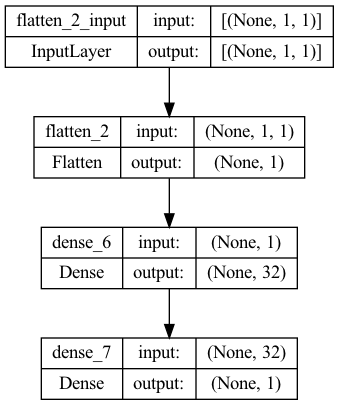
\includegraphics[width=0.6\textwidth]{data/Figures/Neural networks/model_tf1.png}
    \caption{Model architecture.}\label{fig:model_tf1}
\end{figure}

In order to test for the different possible models, we decided to have the batch size, the number of epochs, the number of timesteps and different optimizers as variables in our loop. In addition we tested for both univariate and multivariate models. The batch size is the number of samples that will be propagated through the network, we choose to test for batch sizes between 1 and 104. The number of epochs is the amount of times the model will be trained for each model, we here chose epochs between 10 and 100. The number of time steps we chose to use is a week, 4 weeks, 52 weeks and 104 week. The main reason for this is the hypothesis that the model will perform better if it is able to take the seasonality into account. The optimizers we tested for are Adam and nadam, two of the more accurate optimizers.~\parencite{zaman2021} In conclusion, this resulted in 288 different models.